\documentclass[../report.tex]{subfiles}
\begin{document}
	
\subsection{Normalisation} \label{sec:Z-normalisation}
	The preprocessing technique for normalisation suggested for SAX \citep{sax} is \textit{Z-normalisation}.  That is to normalise the data so that it has a mean ($\bar{x}$) of zero and a standard deviation ($\sigma$) of one.  This is achieved by subtracting the mean from each value and then dividing by the standard deviation.
	
	\begin{equation}
	z = \dfrac{x - \bar{x}}{\sigma}
	\end{equation}
	
	In a closed set of values, this technique often works perfectly fine.  Unfortunately, in this case, the vast majority of data points on seismic recordings are made up of background noise that are often indistinguishable from the events themselves apart from by amplitude.  This means that if background noise is included in the sample from which the mean and standard deviation are taken, then values during the actual event will be over amplified and therefore unsuitable for \textit{SAX} processing.
	
	A further problem introduced by unsupervised normalisation is the tailing off of events.  In the same way that introducing otherwise quiet periods amplifies the peaks of the event, so does including too much of the tail.
	
\begin{figure}[h]
	\begin{subfigure}{\textwidth}
		\centering
		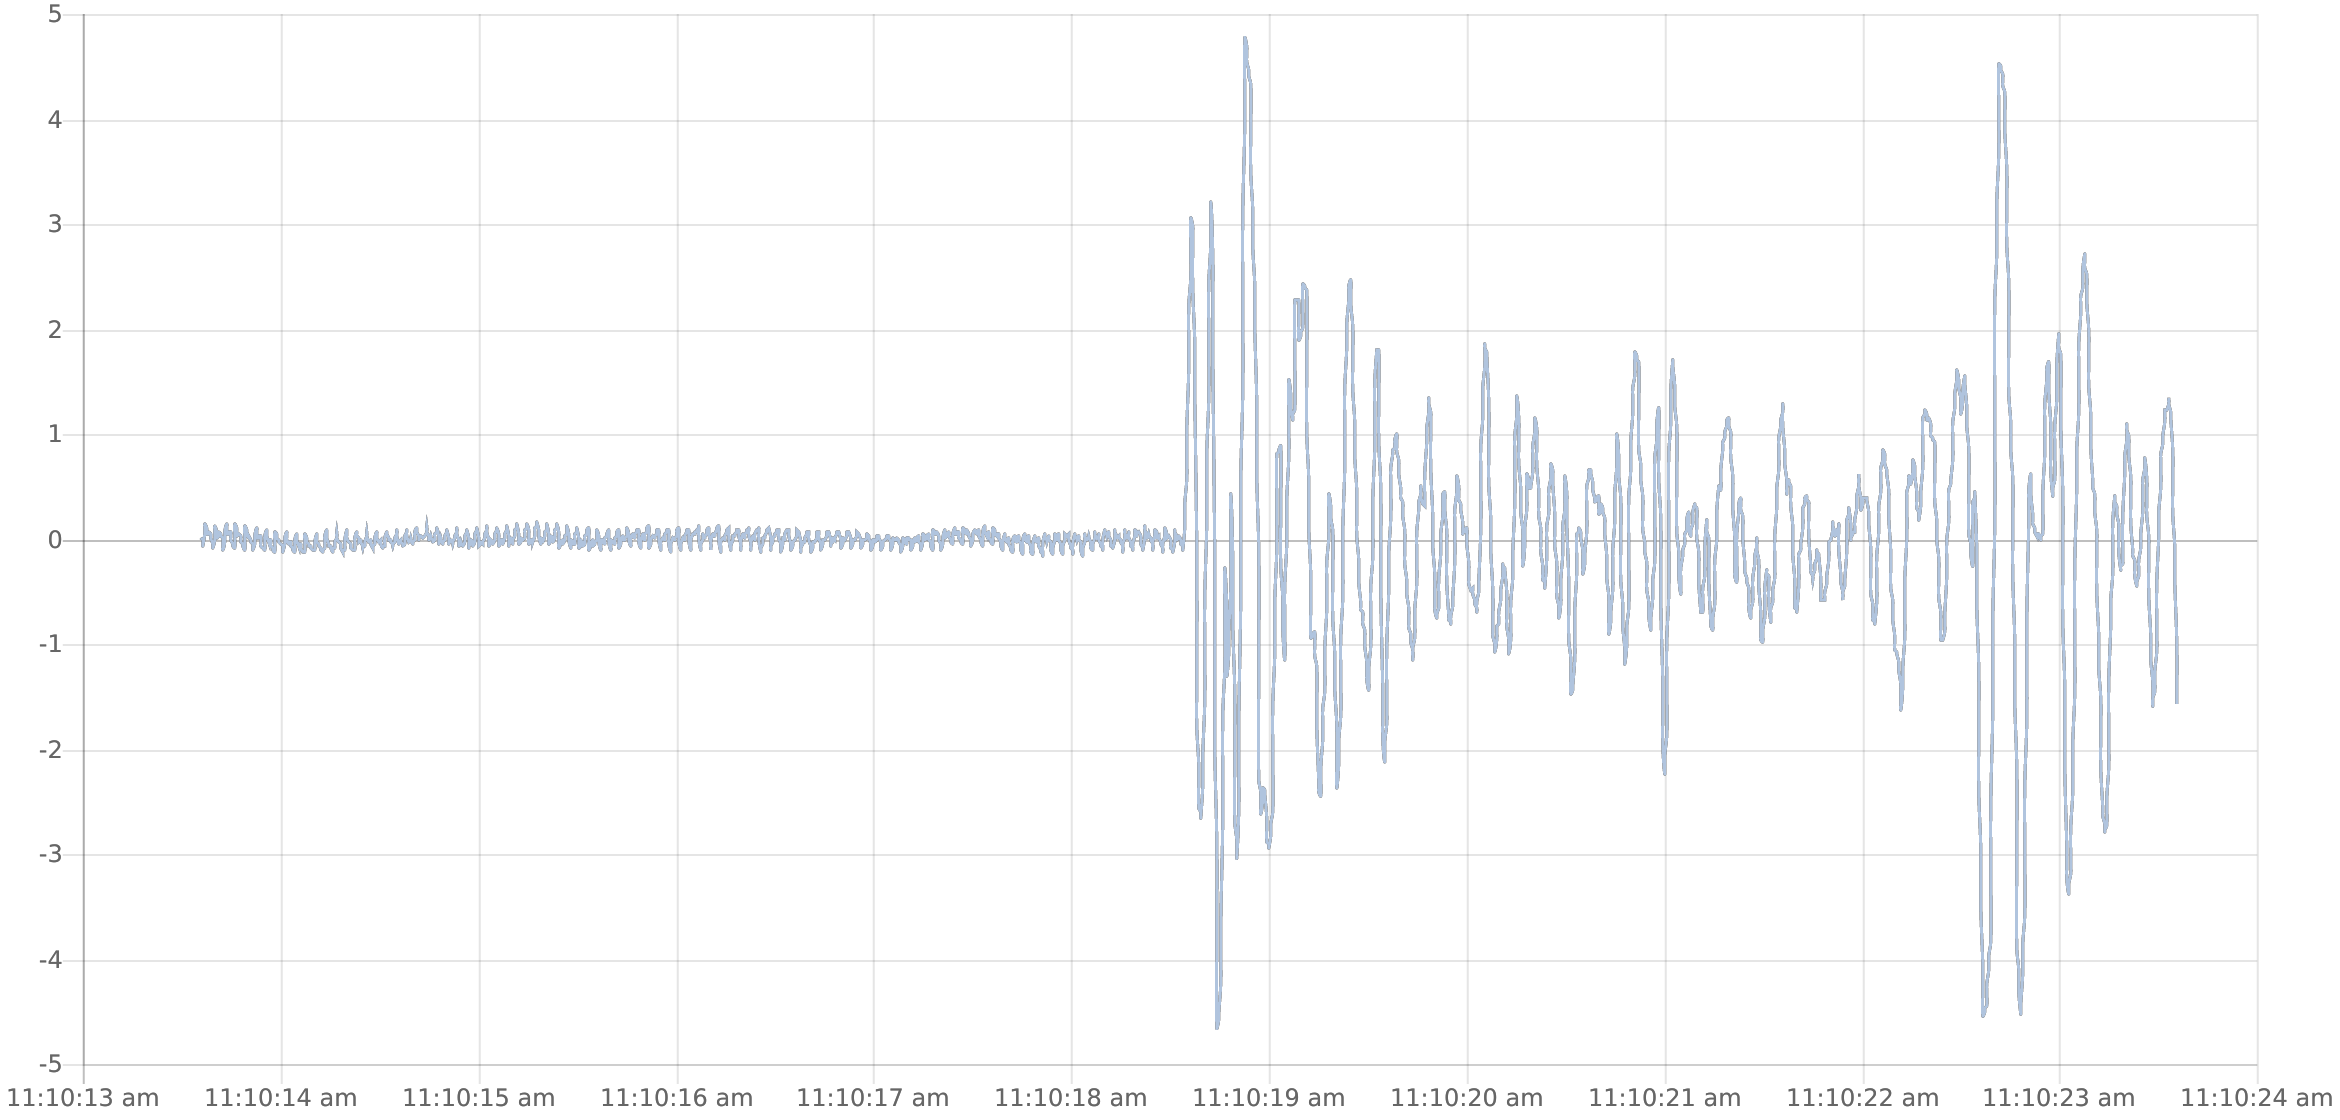
\includegraphics[width=0.7\linewidth]{toSoon}
		\caption[]{With background noise}
	\end{subfigure}
	\begin{subfigure}{\textwidth}
		\centering
		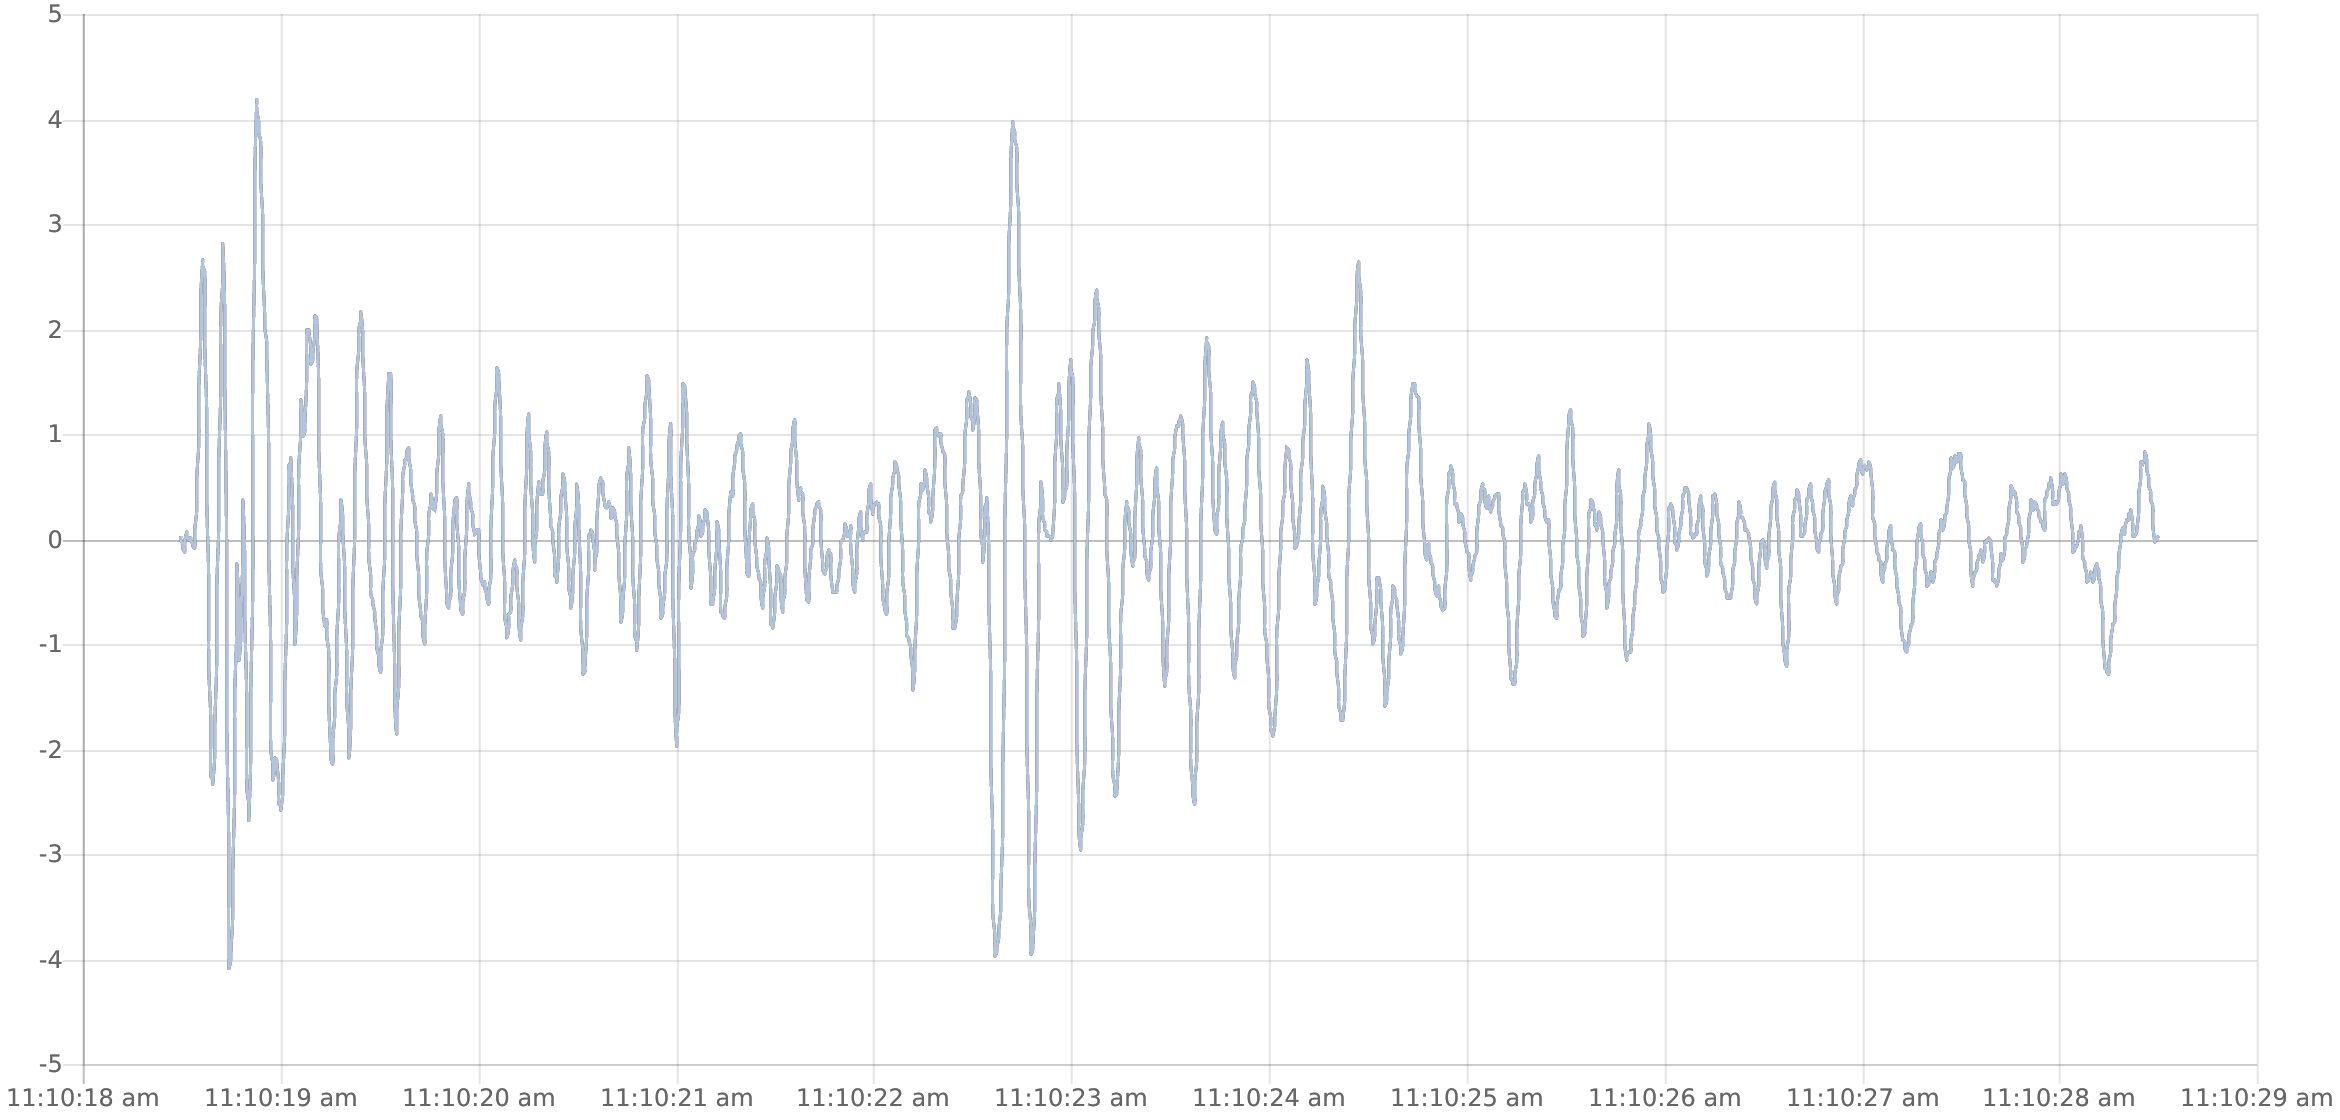
\includegraphics[width=0.7\linewidth]{onTarget}
		\caption[]{Without background noise}
	\end{subfigure}
	\caption{Comparison of normalisation with and without background}
	\label{fig:tosoon}
\end{figure}

	In view of these issues, and because \textit{z-normalisation} is an important part of \textit{SAX processing}, it is essential that only significant data be presented to be normalised for analysis.  To meet this requirement, it is important that the start of the event be relatively accurately estimated and only the first few seconds are treated.  This is also important because we are only interested in profiling \textit{P-waves}. The \textit{S-waves} following a few seconds later interfere with the Z-axis recordings.  This is demonstrated in \cref{fig:tosoon} where if earlier background noise is included in the sample (a) the peaks are normalised a little over 4 where if only the event is included, the peaks are nearer to 5.  When looking at longer time ranges, this effect is amplified significantly rendering the event data meaningless.

\end{document}